
%% bare_conf.tex 
%% V1.2
%% 2002/11/18
%% by Michael Shell
%% mshell@ece.gatech.edu
%% 
%% NOTE: This text file uses UNIX line feed conventions. When (human)
%% reading this file on other platforms, you may have to use a text
%% editor that can handle lines terminated by the UNIX line feed
%% character (0x0A).
%% 
%% This is a skeleton file demonstrating the use of IEEEtran.cls 
%% (requires IEEEtran.cls version 1.6b or later) with an IEEE conference paper.
%% 
%% Support sites:
%% http://www.ieee.org
%% and/or
%% http://www.ctan.org/tex-archive/macros/latex/contrib/supported/IEEEtran/ 
%%
%% This code is offered as-is - no warranty - user assumes all risk.
%% Free to use, distribute and modify.

% *** Authors should verify (and, if needed, correct) their LaTeX system  ***
% *** with the testflow diagnostic prior to trusting their LaTeX platform ***
% *** with production work. IEEE's font choices can trigger bugs that do  ***
% *** not appear when using other class files.                            ***
% Testflow can be obtained at:
% http://www.ctan.org/tex-archive/macros/latex/contrib/supported/IEEEtran/testflow


% Note that the a4paper option is mainly intended so that authors in
% countries using A4 can easily print to A4 and see how their papers will
% look in print. Authors are encouraged to use U.S. letter paper when 
% submitting to IEEE. Use the testflow package mentioned above to verify
% correct handling of both paper sizes by the author's LaTeX system.
%
% Also note that the "draftcls" or "draftclsnofoot", not "draft", option
% should be used if it is desired that the figures are to be displayed in
% draft mode.
%
% This paper can be formatted using the peerreviewca
% (instead of conference) mode.
\documentclass[conference]{IEEEtran}
% If the IEEEtran.cls has not been installed into the LaTeX system files, 
% manually specify the path to it:
% \documentclass[conference]{../sty/IEEEtran} 


% some very useful LaTeX packages include:

%\usepackage{cite}      % Written by Donald Arseneau
                        % V1.6 and later of IEEEtran pre-defines the format
                        % of the cite.sty package \cite{} output to follow
                        % that of IEEE. Loading the cite package will
                        % result in citation numbers being automatically
                        % sorted and properly "ranged". i.e.,
                        % [1], [9], [2], [7], [5], [6]
                        % (without using cite.sty)
                        % will become:
                        % [1], [2], [5]--[7], [9] (using cite.sty)
                        % cite.sty's \cite will automatically add leading
                        % space, if needed. Use cite.sty's noadjust option
                        % (cite.sty V3.8 and later) if you want to turn this
                        % off. cite.sty is already installed on most LaTeX
                        % systems. The latest version can be obtained at:
                        % http://www.ctan.org/tex-archive/macros/latex/contrib/supported/cite/

\usepackage{graphicx}  % Written by David Carlisle and Sebastian Rahtz
                        % Required if you want graphics, photos, etc.
                        % graphicx.sty is already installed on most LaTeX
                        % systems. The latest version and documentation can
                        % be obtained at:
                        % http://www.ctan.org/tex-archive/macros/latex/required/graphics/
                        % Another good source of documentation is "Using
                        % Imported Graphics in LaTeX2e" by Keith Reckdahl
                        % which can be found as esplatex.ps and epslatex.pdf
                        % at: http://www.ctan.org/tex-archive/info/
% NOTE: for dual use with latex and pdflatex, instead load graphicx like:
%\ifx\pdfoutput\undefined
%\usepackage{graphicx}
%\else
%\usepackage[pdftex]{graphicx}
%\fi

% However, be warned that pdflatex will require graphics to be in PDF
% (not EPS) format and will preclude the use of PostScript based LaTeX
% packages such as psfrag.sty and pstricks.sty. IEEE conferences typically
% allow PDF graphics (and hence pdfLaTeX). However, IEEE journals do not
% (yet) allow image formats other than EPS or TIFF. Therefore, authors of
% journal papers should use traditional LaTeX with EPS graphics.
%
% The path(s) to the graphics files can also be declared: e.g.,
% \graphicspath{{../eps/}{../ps/}}
% if the graphics files are not located in the same directory as the
% .tex file. This can be done in each branch of the conditional above
% (after graphicx is loaded) to handle the EPS and PDF cases separately.
% In this way, full path information will not have to be specified in
% each \includegraphics command.
%
% Note that, when switching from latex to pdflatex and vice-versa, the new
% compiler will have to be run twice to clear some warnings.


%\usepackage{psfrag}    % Written by Craig Barratt, Michael C. Grant,
                        % and David Carlisle
                        % This package allows you to substitute LaTeX
                        % commands for text in imported EPS graphic files.
                        % In this way, LaTeX symbols can be placed into
                        % graphics that have been generated by other
                        % applications. You must use latex->dvips->ps2pdf
                        % workflow (not direct pdf output from pdflatex) if
                        % you wish to use this capability because it works
                        % via some PostScript tricks. Alternatively, the
                        % graphics could be processed as separate files via
                        % psfrag and dvips, then converted to PDF for
                        % inclusion in the main file which uses pdflatex.
                        % Docs are in "The PSfrag System" by Michael C. Grant
                        % and David Carlisle. There is also some information 
                        % about using psfrag in "Using Imported Graphics in
                        % LaTeX2e" by Keith Reckdahl which documents the
                        % graphicx package (see above). The psfrag package
                        % and documentation can be obtained at:
                        % http://www.ctan.org/tex-archive/macros/latex/contrib/supported/psfrag/

%\usepackage{subfigure} % Written by Steven Douglas Cochran
                        % This package makes it easy to put subfigures
                        % in your figures. i.e., "figure 1a and 1b"
                        % Docs are in "Using Imported Graphics in LaTeX2e"
                        % by Keith Reckdahl which also documents the graphicx
                        % package (see above). subfigure.sty is already
                        % installed on most LaTeX systems. The latest version
                        % and documentation can be obtained at:
                        % http://www.ctan.org/tex-archive/macros/latex/contrib/supported/subfigure/

%\usepackage{url}       % Written by Donald Arseneau
                        % Provides better support for handling and breaking
                        % URLs. url.sty is already installed on most LaTeX
                        % systems. The latest version can be obtained at:
                        % http://www.ctan.org/tex-archive/macros/latex/contrib/other/misc/
                        % Read the url.sty source comments for usage information.

%\usepackage{stfloats}  % Written by Sigitas Tolusis
                        % Gives LaTeX2e the ability to do double column
                        % floats at the bottom of the page as well as the top.
                        % (e.g., "\begin{figure*}[!b]" is not normally
                        % possible in LaTeX2e). This is an invasive package
                        % which rewrites many portions of the LaTeX2e output
                        % routines. It may not work with other packages that
                        % modify the LaTeX2e output routine and/or with other
                        % versions of LaTeX. The latest version and
                        % documentation can be obtained at:
                        % http://www.ctan.org/tex-archive/macros/latex/contrib/supported/sttools/
                        % Documentation is contained in the stfloats.sty
                        % comments as well as in the presfull.pdf file.
                        % Do not use the stfloats baselinefloat ability as
                        % IEEE does not allow \baselineskip to stretch.
                        % Authors submitting work to the IEEE should note
                        % that IEEE rarely uses double column equations and
                        % that authors should try to avoid such use.
                        % Do not be tempted to use the cuted.sty or
                        % midfloat.sty package (by the same author) as IEEE
                        % does not format its papers in such ways.

\usepackage{amsmath}   % From the American Mathematical Society
                        % A popular package that provides many helpful commands
                        % for dealing with mathematics. Note that the AMSmath
                        % package sets \interdisplaylinepenalty to 10000 thus
                        % preventing page breaks from occurring within multiline
                        % equations. Use:
%\interdisplaylinepenalty=2500
                        % after loading amsmath to restore such page breaks
                        % as IEEEtran.cls normally does. amsmath.sty is already
                        % installed on most LaTeX systems. The latest version
                        % and documentation can be obtained at:
                        % http://www.ctan.org/tex-archive/macros/latex/required/amslatex/math/



% Other popular packages for formatting tables and equations include:

\usepackage{array}
% Frank Mittelbach's and David Carlisle's array.sty which improves the
% LaTeX2e array and tabular environments to provide better appearances and
% additional user controls. array.sty is already installed on most systems.
% The latest version and documentation can be obtained at:
% http://www.ctan.org/tex-archive/macros/latex/required/tools/

% Mark Wooding's extremely powerful MDW tools, especially mdwmath.sty and
% mdwtab.sty which are used to format equations and tables, respectively.
% The MDWtools set is already installed on most LaTeX systems. The lastest
% version and documentation is available at:
% http://www.ctan.org/tex-archive/macros/latex/contrib/supported/mdwtools/


% V1.6 of IEEEtran contains the IEEEeqnarray family of commands that can
% be used to generate multiline equations as well as matrices, tables, etc.


% Also of notable interest:

% Scott Pakin's eqparbox package for creating (automatically sized) equal
% width boxes. Available:
% http://www.ctan.org/tex-archive/macros/latex/contrib/supported/eqparbox/

\usepackage{multirow}
\usepackage[table]{xcolor}

% Notes on hyperref:
% IEEEtran.cls attempts to be compliant with the hyperref package, written
% by Heiko Oberdiek and Sebastian Rahtz, which provides hyperlinks within
% a document as well as an index for PDF files (produced via pdflatex).
% However, it is a tad difficult to properly interface LaTeX classes and
% packages with this (necessarily) complex and invasive package. It is
% recommended that hyperref not be used for work that is to be submitted
% to the IEEE. Users who wish to use hyperref *must* ensure that their
% hyperref version is 6.72u or later *and* IEEEtran.cls is version 1.6b 
% or later. The latest version of hyperref can be obtained at:
%
% http://www.ctan.org/tex-archive/macros/latex/contrib/supported/hyperref/
%
% Also, be aware that cite.sty (as of version 3.9, 11/2001) and hyperref.sty
% (as of version 6.72t, 2002/07/25) do not work optimally together.
% To mediate the differences between these two packages, IEEEtran.cls, as
% of v1.6b, predefines a command that fools hyperref into thinking that
% the natbib package is being used - causing it not to modify the existing
% citation commands, and allowing cite.sty to operate as normal. However,
% as a result, citation numbers will not be hyperlinked. Another side effect
% of this approach is that the natbib.sty package will not properly load
% under IEEEtran.cls. However, current versions of natbib are not capable
% of compressing and sorting citation numbers in IEEE's style - so this
% should not be an issue. If, for some strange reason, the user wants to
% load natbib.sty under IEEEtran.cls, the following code must be placed
% before natbib.sty can be loaded:
%
% \makeatletter
% \let\NAT@parse\undefined
% \makeatother
%
% Hyperref should be loaded differently depending on whether pdflatex
% or traditional latex is being used:
%
%\ifx\pdfoutput\undefined
%\usepackage[hypertex]{hyperref}
%\else
%\usepackage[pdftex,hypertexnames=false]{hyperref}
%\fi
%
% Pdflatex produces superior hyperref results and is the recommended
% compiler for such use.


% *** Do not adjust lengths that control margins, column widths, etc. ***
% *** Do not use packages that alter fonts (such as pslatex).         ***
% There should be no need to do such things with IEEEtran.cls V1.6 and later.

% Reminder: the "draftcls" or "draftclsnofoot", not "draft", class option
% should be used if it is desired that the figures are to be displayed while
% in draft mode.

% An example of a floating figure using the graphicx package.
% Note that \label must occur AFTER (or within) \caption.
% For figures, \caption should occur after the \includegraphics.
%
%\begin{figure}
%\centering
%\includegraphics[width=2.5in]{myfigure}
% where an .eps filename suffix will be assumed under latex, 
% and a .pdf suffix will be assumed for pdflatex
%\caption{Simulation Results}
%\label{fig_sim}
%\end{figure}


% An example of a double column floating figure using two subfigures.
%(The subfigure.sty package must be loaded for this to work.)
% The subfigure \label commands are set within each subfigure command, the
% \label for the overall fgure must come after \caption.
% \hfil must be used as a separator to get equal spacing
%
%\begin{figure*}
%\centerline{\subfigure[Case I]{\includegraphics[width=2.5in]{subfigcase1}
% where an .eps filename suffix will be assumed under latex, 
% and a .pdf suffix will be assumed for pdflatex
%\label{fig_first_case}}
%\hfil
%\subfigure[Case II]{\includegraphics[width=2.5in]{subfigcase2}
% where an .eps filename suffix will be assumed under latex, 
% and a .pdf suffix will be assumed for pdflatex
%\label{fig_second_case}}}
%\caption{Simulation results}
%\label{fig_sim}
%\end{figure*}



% An example of a floating table. Note that, for IEEE style tables, the 
% \caption command should come BEFORE the table. Table text will default to
% \footnotesize as IEEE normally uses this smaller font for tables.
% The \label must come after \caption as always.
%
%\begin{table}
%% increase table row spacing, adjust to taste
%\renewcommand{\arraystretch}{1.3}
%\caption{An Example of a Table}
%\label{table_example}
%\begin{center}
%% Some packages, such as MDW tools, offer better commands for making tables
%% than the plain LaTeX2e tabular which is used here.
%\begin{tabular}{|c||c|}
%\hline
%One & Two\\
%\hline
%Three & Four\\
%\hline
%\end{tabular}
%\end{center}
%\end{table}

% correct bad hyphenation here
\hyphenation{op-tical net-works semi-conduc-tor IEEEtran}

\linespread{1}
\setlength{\parskip}{0cm}
\setlength{\parindent}{1em}
\setlength{\parskip}{0pt}
\setlength{\parsep}{0pt}


\begin{document}

% paper title
\title{Image Inpainting using Multi-Scale Learned Dictionaries in the Wavelet Domain}


% author names and affiliations
% use a multiple column layout for up to three different
% affiliations
%\author{\authorblockN{Marica Bertarini}
%\authorblockA{Department of Computer Science\\
%ETH, Zurich\\
%Switzerland\\
%maricab@student.ethz.ch}
%\and
%\authorblockN{Ruifeng Xu}
%\authorblockA{Department of Computer Science\\
%ETH, Zurich\\
%Switzerland\\
%ruxu@student.ethz.ch}
%\and
%\authorblockN{Sevgi Kaya\\}
%\authorblockA{Department of Computer Science\\
%ETH, Zurich\\
%Switzerland\\
%skaya@student.ethz.ch}}


% avoiding spaces at the end of the author lines is not a problem with
% conference papers because we don't use \thanks or \IEEEmembership


% for over three affiliations, or if they all won't fit within the width
% of the page, use this alternative format:
% 
\author{\authorblockN{Marica Bertarini,
Sevgi Kaya and 
Ruifeng Xu}
\authorblockA{\{maricab\textbar skaya\textbar ruxu\}@student.ethz.ch\\
Department of Computer Science, ETH Zurich, Switzerland}}


% use only for invited papers
%\specialpapernotice{(Invited Paper)}

% make the title area
\maketitle

\begin{abstract}
Recent studies on sparse and redundant signal representations have shown trends to merge dictionary learning with multi-scale analytical frameworks such as wavelet or time-to-frequency transformations. Because most natural signals can be expressed at multiple scales, such approach is appealing by combining the advantages of fitting dictionaries more finely to real data and the expressiveness of multi-scale representations. In this paper, we extend the work \cite{multiscaleDictLearning} on multi-scale dictionary learning to the paradigm of image inpainting and compare our result to existing techniques to demonstrate the effectiveness of our approach. We also identify the impact of different parameters of our model on our result through experiments.
\end{abstract}

% no keywords

% For peer review papers, you can put extra information on the cover
% page as needed:
% \begin{center} \bfseries EDICS Category: 3-BBND \end{center}
%
% for peerreview papers, inserts a page break and creates the second title.
% Will be ignored for other modes.
\IEEEpeerreviewmaketitle

\section{Introduction}
Under the assumption that most natural signals can be sparsely represented as a linear combination of atom signals, various state-of-the-art sparsity-based models have been proposed in recent years \cite{elad09}. Since obtaining exact sparse representations is NP-hard, approximate solutions such as Matching Pursuit (MP) \cite{mallat}, Orthogonal Matching Pursuit (OMP) \cite{pati} and FOCUSS \cite{focuss} are widely adopted. The accuracy of sparse coding using such algorithms requires an appropriate dictionary. Generally, a dictionary can be constructed either by utilizing  analytical frameworks or through explict learning process from real data. The former approach avoids explicit matrix representation; while the latter one leads to better fitted dictionary at the expense of increased computation cost \cite{multiscaleDictLearning}. 

 For image processing in particular, it has been proven in \cite{husoy} that introducing multi-scale analysis to applications such as image denoising and compression improves the visual quality of the reconstructed image. Inspired by \cite{multiscaleDictLearning}, we propose to extend their model to image inpainting by learning and applying multi-scale dictionaries locally in the wavelet domain. Because images are decomposed into multiple scales, our approach can potentially capture and represent the underlying structure of the data more effectively.

The paper is organized as follow. In section \ref{related}, we describe works related to our model. In section \ref{contribution}, we state our contributions and present our model for image inpanting. Section \ref{exp} presents the experiments we conduct and compares our result to other existing inpainting techniques. Sections \ref{discussion} discusses the result and section \ref{conclusion} concludes this paper.

\section{Related Works}\label{related}
Learning multi-scale overcomplete dictionaries have been extensively studied in image inpainting for many years. Multi-scale learning is generally achieved by applying wavelet pyramids on the training data. In \cite{pati} and \cite{mallat}, the sparsity is induced using a-priori on wavelet coefficients which leads to slightly sparser signal bases. However, enforcing the sparsity by setting a prior distribution requires complex procedures to reveal the underlying statistical structure of the data. The generalized algorithm for learning such multi-scale dictionaries is proposed in [5] where a joint global dictionary is trained in a Quadtree structure with different sizes for blocks and atoms. However, computational complexity of Quadtree data structure limits the usage of such methods on large datasets.

K-SVD \cite{ksvd} is one of the most successful strategies to adapt dictionaries for sparse signal representations. K-SVD learns dictionaries in a straightforward and effective way by updating the learned signal atoms from the previous iteration with the sparse coding of the current data samples. The convergence is accelerated by the simultaneous update of the sparse coefficients and dictionary atoms. The sparse coding stage puts little constraint on the approximation algorithm and most pursuit algorithms such as MP and OMP can be used.

\begin{figure}[h]
\centering
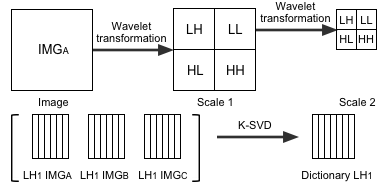
\includegraphics[width=0.45\textwidth]{learning_schema}
\caption{Training images transformed with wavelet transformation and dictionary learning example in the wavelet domain.}
\label{dictLearningFigure}
\end{figure}

Our approach is inspired by the work \cite{multiscaleDictLearning}, where dictionaries are learned from the wavelet decompositions of images using K-SVD \cite{ksvd}. Figure \ref{dictLearningFigure} illustrates the process of dictionary learning. First, training images are recursively decomposed into \emph{3S+1} bands using a chosen 2D wavelet transformation, where \emph{S} represents the total level (scale) of decomposition. Then for the same band of all training images, maximally-overlapping patches are extracted, concatenated and K-SVD is run per band to learn \emph{3S+1} sub-dictionaries. This model provides specific sparse representation with computationally inexpensive local operations on high-dimensional signal groups and hence, it further reduces the spatial redundancy of wavelet coefficients. However, the study only applies the learned dictionary to \textit{M-term} approximation of noisy images and compressed sensing scenarios, and hence it involves no pixel-level inference to fill the missing pixels in the images as in our case. Furthermore, their denoising result has not revealed significant improvement compared to the single-scale K-SVD and the effect of different wavelet tranformation and the decomposition level is not extensively studied.

In \cite{imageInpaintingAlgo}, the model from \cite{multiscaleDictLearning} is applied to image inpainting where an image is reconstructed using a global dictionary in the image domain. The global dictionary is built from all sub-dictionaries trained in the wavelet domain. Our model differs from \cite{imageInpaintingAlgo} by learning and applying the dictionaries for image inpainting locally in each band. 


\section{Our Contribution}\label{contribution}
In this project, we extend the model in \cite{multiscaleDictLearning} to the paradigm of image inpainting. After implementing our model, we conduct experiments to demonstrate the effectiveness of our approach by comparing our result to other inpainting techniques. We also study the impact of different parameters of our model, e.g. pixel inferring methods, dictionary size and training set selection, etc. on the result of inpainting. In the following section, we describe the extensions we made to the model in \cite{multiscaleDictLearning} in order to adapt it to inpainting tasks.

\subsection{Inpainting Algorithm}
To learn a dictionary for sparse and redundant representations, we follow the algorithm proposed in \cite{multiscaleDictLearning}. Different from \cite{imageInpaintingAlgo}, our model not only learns but also applies dictionaries locally in each wavelet decomposition band.

However, one challenge in conducting sparse coding in the wavelet domain is that information about the missing pixels is lost and it is unclear how the missing pixels in a masked image are located in the decompositions. We therefore propose to prefill the missing pixels of a masked image using some primitive inferring methods before applying wavelet decomposition to it, which is described in more detail in \ref{inferringMethods}, and then apply sparse coding on the prefilled image.

Consider a masked image $I$ with missing pixels, the first step of our reconstruction process is to prefill the missing pixels to obtain $I_f$. We then recursively decompose $I_f$ into to \textit{b} bands using wavelet transform $W_A$. For each band, we find the sparse representation using a pursuit algorithm. Note that by prefilling the missing pixels, our sparse coding process assumes the whole image as non-missing. Also, to further capture the dependencies among patches, we adopted horizontal half-overlapping patch extraction strategy. Given the $p$-th patch $[W_AI_f]^{p}_b$ from band $b$, it will be represented by at most $l$ non-zero coefficients as follow
\begin{equation}
x^{*} \in \operatorname{arg\,min}_x \|[W_AI_f]^{p}_b-D_bx^{p}_b\|_2
\quad \text{s.t.} \quad \|x^{p}_b\|_0 \leq l
\end{equation}
This is repeated for all patches $p$ extracted from all bands $b$. The next step is to reconstruct each band $b$ using the sparse representation coefficients $x^{p}_b$ for dictionary $D_b$ and apply inverse wavelet transform $W_s$ to the reconstructed bands to obtain $I_{rec}$. The final operation of reconstruction is to replace the missing pixels in $I$ by taking the corresponding ones from $I_{rec}$.

\begin{table}
\centering
\renewcommand{\arraystretch}{1.1}
\caption{A Summary of Different Inferring Methods}
\label{inferringMethodsTable}
\begin{tabular}{m{2cm} m{5.5cm}}
\hline
\rowcolor{lightgray}\multicolumn{1}{c}{Method Name} & \multicolumn{1}{c}{Neigborhood Definition}\\
\hline
\multicolumn{1}{c}{Patch Mean (Median)} & Mean (median) of the corresponding patch \\
\hline
\multicolumn{1}{c}{4 Diagonal (HV)} & The 4 points at the diagonal (horizontal \& vertical) corners\\
\hline
\multicolumn{1}{c}{4 Diagonal (HV) First} & The 4 points at diagonal (horizontal \& vertical) corners first. If they are all missing, the 4 points at the horizontal \& vertical (diagonal) corners before incrementing the distance limit \\
\hline
\multicolumn{1}{c}{8 Frame} & The 8 points at the diagonal, horizontal \& vertical corners \\
\hline
\multicolumn{1}{c}{Diamond (Square)} & The diamond (square) bounded by the 4 horizontal \& vertical  (diagonal) corners \\
\hline
\end{tabular}
\end{table}

\subsection{Inferring Missing Pixels}\label{inferringMethods}
Intuitively, our pixel inferring methods utilize local similarities existing in most natural images. The grayscale value of a missing pixel is estimated by investigating the non-missing pixels in its vicinity. In this study, a total of nine methods are attempted and they can be classified into two categories, i.e. \textit{patch-based} and \textit{pixel-based} methods. Next, the general principle of these methods are introduced with a summary of different methods presented in Table \ref{inferringMethodsTable}. The performance and impact of them are discussed in section \ref{exp}.

For patch-based methods, an image with missing pixels is first divided into patches. For all missing pixels in a patch, their grayscale values are estimated using either the mean or the median of the non-missing pixels in that patch. On the other hand, pixel-based methods provide more fine-grained estimation by considering each missing pixel individually in an iterative manner. Methods of this category scan the neighborhood of each missing pixel bounded by an increasing distance limit starting from 1 and ending at a threshold value. In each iteration, if any non-missing pixel is discovered, the average of those pixels are used as an approximation of the missing pixel and the process continues to the next missing pixel. Otherwise, the distance limit is incremented by 1 and a bigger neighbourhood is searched. Therefore, the behaviour of different methods in this category relies only on the definition of  neighbourhood. Note that in either case, a default value of 0.5 is used whenever a patch or the neighbourhood of a missing pixel consists completely of missing pixels.

\section{Experiments}\label{exp}
This section discusses most of the experiments we have conducted to study, test and improve our model. The accuracy is measured in terms of root-mean-squared error (RMSE) and the efficiency in terms of running time. A dataset of 64 images \cite{dataset} of size 512x512 pixels and a textual mask that is partly shown in Figure \ref{image_comparison} are used.

\subsection{Optimizations}

\subsubsection{Comparing inferring missing pixels methods}
This experiment compares the performance and impact of different pixel inferring methods we have implemented. The result is shown in Figure \ref{inferringComparisonPlot}. The RMSE is not measured immediately after the application of inferring methods. Instead, it is measured at the end of the whole inpainting process as described in \ref{inferringMethods}. The method \textit{8 frame} is chosen as it has the lowest execution time compared to \textit{4 diagonal first} and \textit{Diamond} which give similar result in terms of RMSE and standard deviation (STD).
\begin{figure}[h]
\centering
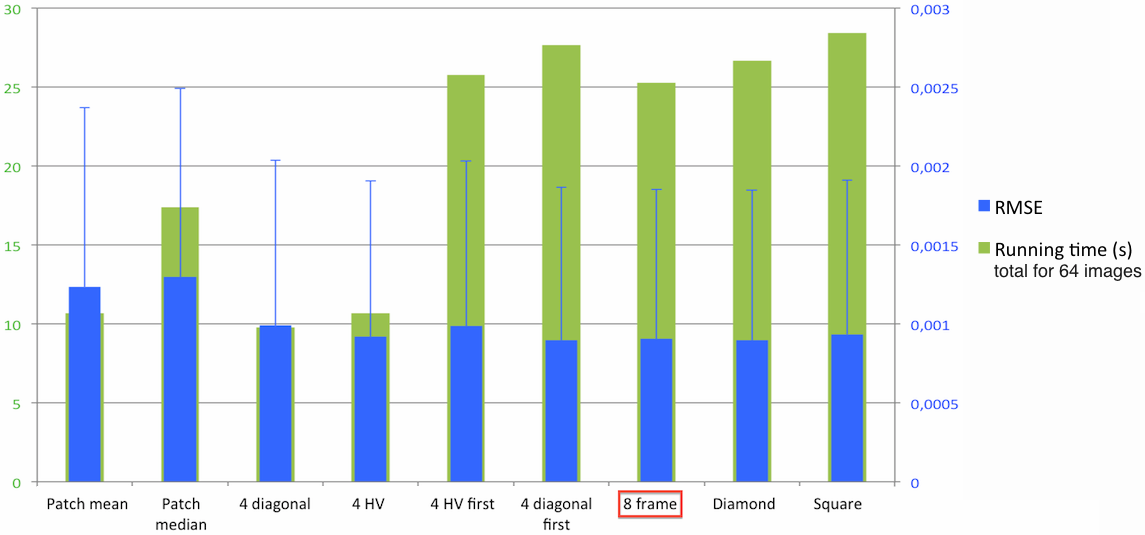
\includegraphics[width=0.45\textwidth]{filling_methods_plot_smaller}
\caption{Comparison of Different Pixel Inferring Methods for 64 Images}
\label{inferringComparisonPlot}
\end{figure}

\subsubsection{Choosing the optimal maximum number of iterations for OMP}
We have implemented both MP and OMP. OMP has been chosen since it leads to more accurate result although it takes longer time. In choosing the optimal maximum number of iterations, we first considered 6 iterations as a reference value based on \cite{imageInpaintingAlgo} and we have measured RMSE and running time for different values around it. Figure \ref{iterations_omp}a shows that RMSE decreases and running time increases as the number of iterations grows. This is expected since multi-scale transform is energy preserving \cite{multiscaleDictLearning}, therefore, this optimization problem in the multi-scale wavelet domain is still convex. We also choose 6 as the optimal value by trading off the accuracy and running time.

\begin{figure}[h]
\centering
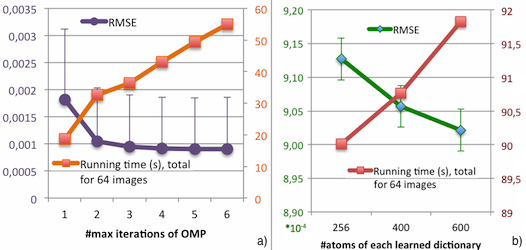
\includegraphics[width=0.45\textwidth]{atoms_omp_together_small}
\caption{RMSE and running time of sparse coding as (a) the number of iterations of OMP grows and (b) the number of dictionary atoms increases for 64 images}
\label{iterations_omp}
\end{figure}

\subsection{Dictionary Learning}
The following experiments aim to exam the impact of different learned dictionaries on RMSE and inpainting running time. All the dictionaries are learnt for 1 scale with 100 iterations \cite{imageInpaintingAlgo} for K-SVD from 15 images. A maximum number of 6 iterations for OMP is used and horizontal half-overlapping patches of size 8x8 pixels from each sub-band are extracted.

\subsubsection{Increasing dictionary size}
Figure \ref{iterations_omp}b shows that as the number of atoms in the learned dictionaries increases, RMSE decreases since more features are captured in the dictionaries. In contrast, the running time increases because larger matrices are involved. As a trade-off, we choose to use 400 atoms instead of 256 atoms for dictionary size, although the reduction in terms of RMSE is small.

\subsubsection{Ineffective trials}
Other minor experiments have been performed. They have not significantly decreased the RMSE, probably because few levels of each factor have been used due to time constraints. Some examples are 1 vs 2 scale dictionary learning, \textit{Haar} vs \textit{discrete Meyer} wavelet, different dictionary initializations strategies (e.g. random samples vs DCT), increasing the size of the training set, and learning from whole images vs choosing random patches from training set.
\subsection{Comparing with Baselines} \label{baselinesSection}
In this sub-section, we describe other inpainting methods we implement as baselines to compare and evaluate our approach.
\subsubsection{Sparse Coding with Overcomplete DCT} \label{dct}
It solves the image inpainting problem by finding a sparse representation of each non-overlapping patch of the masked image in the overcomplete DCT dictionary. Therefore, the missing pixels in the masked image are replaced by the corresponding ones in the reconstruction.
\subsubsection{K-SVD in the image domain for inpainting}
It learns a dictionary in the signal domain using K-SVD \cite{ksvd} from a training set and then it uses the learned dictionary as explained in \ref{dct} in place of the DCT dictionary.
\subsubsection{Singular Value Decomposition (SVD)}
SVD is applied to the masked image after its missing pixels are inferred by using the \textit{Patch Mean} method (see Table \ref{inferringMethodsTable}). It leads to the best RMSE compared to the others inferring methods. The model selection parameter concerning the number of singular values kept to compute the reconstruction is found via K-fold Cross Validation. The missing pixels in the masked image are replaced by the corresponding ones in the reconstruction.

 \begin{figure}[h]
\centering
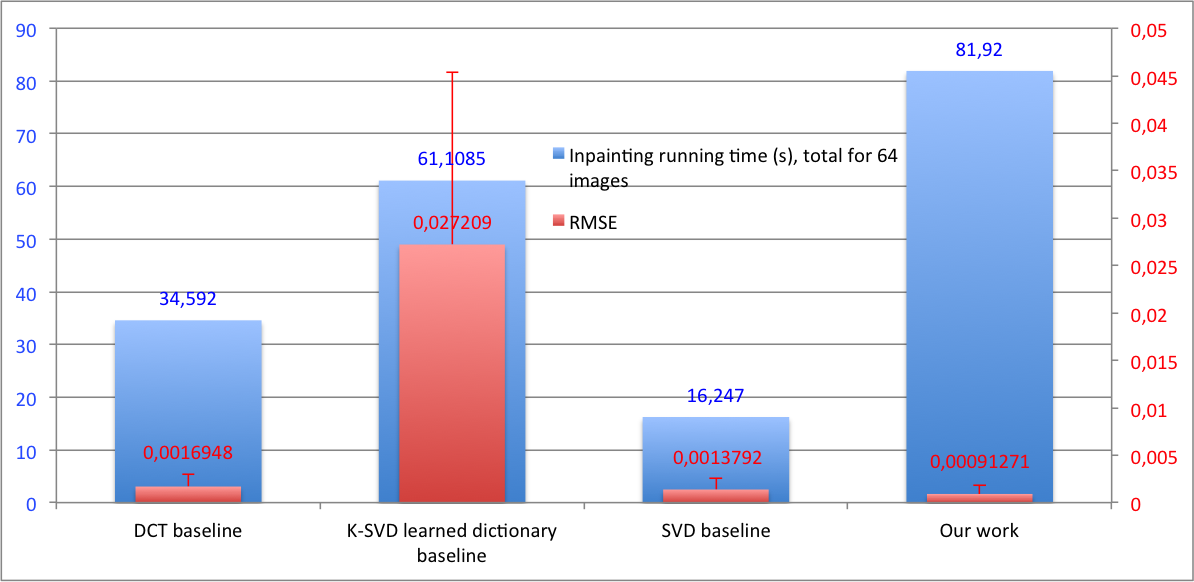
\includegraphics[width=0.45\textwidth]{baselines_comparison}
\caption{RMSE and inpainting running time of three different baselines and our work, measured on 64 images}
\label{baselines_graph}
\end{figure}
 

 The histogram in Figure \ref{baselines_graph} compares the models described above with our work. DCT, K-SVD baseline and our work learn or/and use dictionaries of 256 atoms and share the same parameter values to solve the sparse coding problem using OMP. The two baselines could obtain of course better result with bigger dictionaries, however the size is kept fixed to perform a meaningful comparison with our work. On the other hand, the SVD baseline, which is a completely different model, has been optimized as much as possible for comparison. 

  The running time shown in the figure refers only to the reconstruction process, which means the dictionary learning time is excluded. It is evident that our model takes significant longer time to restore images: this is easily understandable with respect to SVD since the latter infers the missing pixels exactly as our project does at the beginning, then it only performs a Singular Value Decomposition. As for DCT and K-SVD baselines, the inpainting execution time is shorter than our as they solve the sparse coding problem with a dictionary of 256 atoms only once, whereas our model solves it $b$ times. Moreover, the running time of DCT and K-SVD baselines which use the same inpainting model and dictionaries of the same size, are different because different patch sizes are used during the experiments, i.e. 16x16 and 8x8 pixels respectively.  
  
  With regard to RMSE, the graph shows that our model outperforms all the other approaches. This is particularly important, especially when compared to the K-SVD baseline, as it proves that learning multi-scale dictionaries in the wavelet domain is better than learning single-scale dictionary of equal size in the image domain. Another advantage of our approach to the K-SVD baseline is that our learning procedure is parallelizable since it learns one dictionary per band independently. On the contrary, K-SVD in the signal domain can learn only one dictionary at a time.

\begin{figure}[h]
\centering
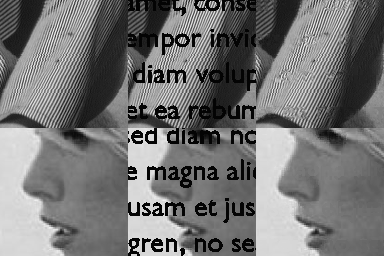
\includegraphics[width=0.45\textwidth]{image_comparison}
\caption{Original (left), masked (middle) and reconstructed image (right) of the worst (up) and best (down) reconstruction cases out of 64 images}
\label{image_comparison}
\end{figure}

\section{Discussion}\label{discussion}
In order to gain better understanding of our approach, we visualized and examined the reconstructed images from the dataset. Figure \ref{image_comparison} shows part of the two reconstructed images. The upper row and the lower row contain the reconstructed image with the highest and the lowest RMSE respectively. From the figure we can see that our approach performs relatively better on facial images than patterns. This is probably due to the fact that we used much fewer texture images in our training set than human faces and smooth patches. Nevertheless, the experiment results indicate that our reconstructions of general images outperform the ones from all baselines.

Furthermore, the main weakness of our approach is the running time given that our sparse coding process is run on each decomposed band. This effect, however, can be alleviated with the support of parallel programming. In fact, we have implemented a parallel version of our work that finds the sparse representation of all the $b$ bands concurrently. This has halved the running time, which is promising since most modern computers natively support parallel computing and this could lead to a more competitive execution time.

\section{Conclusion}\label{conclusion}
In this work, we present an extension to the K-SVD image inpainting algorithm by combining pixel inferring methods with multi-scale learned dictionary in the wavelet domain. The results, especially in terms of accuracy, reveal the potential of training dictionaries in multi-scale analytical frameworks.

% conference papers do not normally have an appendix

% use section* for acknowledgement
% \section*{Acknowledgment}
% optional entry into table of contents (if used)
%\addcontentsline{toc}{section}{Acknowledgment}
% The authors would like to thank...

% trigger a \newpage just before the given reference
% number - used to balance the columns on the last page
% adjust value as needed - may need to be readjusted if
% the document is modified later
%\IEEEtriggeratref{8}
% The "triggered" command can be changed if desired:
%\IEEEtriggercmd{\enlargethispage{-5in}}

% references section
% NOTE: BibTeX documentation can be easily obtained at:
% http://www.ctan.org/tex-archive/biblio/bibtex/contrib/doc/

% can use a bibliography generated by BibTeX as a .bbl file
% standard IEEE bibliography style from:
% http://www.ctan.org/tex-archive/macros/latex/contrib/supported/IEEEtran/bibtex
%\bibliographystyle{IEEEtran.bst}
% argument is your BibTeX string definitions and bibliography database(s)
%\bibliography{IEEEabrv,../bib/paper}
%
% <OR> manually copy in the resultant .bbl file
% set second argument of \begin to the number of references
% (used to reserve space for the reference number labels box)
\begin{thebibliography}{1}
\bibitem{elad09}A. M. Bruckstein, D. L. Donoho, and M. Elad, \emph{From Sparse Solutions of Systems of Equations to Sparse Modeling of Signals and Images}, SIAM Rev., vol. 51, no. 1, pp. 34–81, 2009
\bibitem{pati} Y. C. Pati, R. Rezaiifar, and P. S. Krishnaprasad, \emph{Or- thogonal Matching Pursuit: Recursive Function Ap- proximat ion with Applications to Wavelet Decompo- sition}, Asilomar Conf. Signals, Syst. Comput. IEEE, pp. 40–44, 1993
\bibitem{mallat} S. Mallat and Z. Zhang, \emph{Matching Pursuits With Time-Frequency Dictionaries}, IEEE Trans. Signal Process., vol. 41, no. 12, pp. 3397–3415, 1993
\bibitem{focuss}I. F. Gorodnitsky and B. D. Rao, \emph{Sparse signal re- construction from limited data using FOCUSS: a re- weighted minimum norm algorithm}, IEEE Trans. Signal Process., vol. 45, no. 3, pp. 600–616, 1997
\bibitem{husoy} K. Engan, S. O. Aase, and J. H. Husoy, \emph{Method of Op- timal Directions for Frame Design}, in IEEE Int. Conf. Acoust. Speech, Signal Process., pp. 2443–2446, 1999
\bibitem{ksvd}
M. Aharon, M. Elad, and A. Bruckstein, \emph{K-SVD: Design of Dictionaries for Sparse Representation}, IEEE Trans. Signal Process., vol. 54, no. 11, pp. 4311-4322, 2006
\bibitem{multiscaleDictLearning}
B. Ophir, M. Lustig, and M. Elad, \emph{Multi-Scale Dictionary Learning using Wavelets}, IEEE Trans. Signal Process., vol. 5, no. 5, pp. 1014-1024, 2011
\bibitem{imageInpaintingAlgo}
J.~Liu, X.~Ma, \emph{An improved image inpainting algorithm based on multi-scale dictionary learning in wavelet domain}, Signal Processing, Communication and Computing (ICSPCC), 2013 IEEE International Conference, pp. 1-5, 2013
\bibitem{dataset}
Gaox, \emph{"Image-inpainting data"}. Internet: https://github.com/gaox/image-inpainting/tree/master/data, Jun. 22, 2012 [Jun. 19, 2014]

\end{thebibliography}


% that's all folks
\end{document}

